% ZhCvGo15.tex      pdflatex ZhCvGo15

% Diffuse globally, compute locally: a cyclist tale
% Tingnan Zhang, Daniel I. Goldman and Predrag Cvitanovi\'c

                  %%   logical setup, no need to edit %%%%%%%%%%
                  \newif\ifpaper \paperfalse \newif\ifPDF \PDFtrue %%
                  \newif\ifboyscout %%
                  \boyscouttrue %% commented, WWW/drafts %%
%%%% Toggle between draft and public versions
% \boyscoutfalse % public, for hyperlinked pdf

% Predrag                       2015-11-19
% Tingnan                       2015-11-

        \ifboyscout
\documentclass[aps,pre,
                showpacs,
                twocolumn,
                %preprint,      %uncomment for double spacing
                groupedaddress,
                floatfix]{revtex4-1}
        \else
\documentclass[pre,aps,
                twocolumn,
                showpacs,
                superscriptaddress,
                groupedaddress,
                floatfix,
                hyperref]{revtex4-1}
        \fi
%   REVTeX 4 Version 4.1r August 2010
%   Phys. Rev. appearance, change preprint to twocolumn.  Choose pra,
%   prb, prc, prd, pre, prl, prstab for journal Add
%   'draft' option to mark overfull boxes with black boxes Add
%   'showpacs' option to make PACS codes appear Add 'showkeys' option
%   to make keywords appear
% Use the \preprint command to place your local institutional report
% number in the upper righthand corner of the title page in preprint
% mode.  Multiple \preprint commands are allowed.  Use the
% 'preprintnumbers' class option to override journal defaults to
% display numbers if necessary \preprint{}

\input ../inputs/setupSveZha
\input ../inputs/editsDasbuch %% editing comments, DasBuch style
\input ../inputs/def %% do not edit; update from dasbuch/book/inputs/def.tex
\input ../inputs/defsSveZha %% all diffusion project edits: \renewcommand, etc

\begin{document}

\title{Discrete factorization of deterministic diffusion}
\TZ{2015-11-02}{Dan is not a big fan of the title. Do we have a more formal version?}
\author{Tingnan Zhang}
\author{Daniel I. Goldman}
\author{Predrag Cvitanovi\'c}

\email[]{predrag@gatech.edu}
\homepage[]{ChaosBook.org}
\thanks{NSF DMS-1211827}
\affiliation{School of Physics, Georgia Institute of Technology, Atlanta GA}
%   Group addresses by affiliation; use superscriptaddress for long
%   author lists, or if there are many overlapping affiliations.
% repeat the \author .. \affiliation etc. as needed \email, \thanks,
% \homepage, \altaffiliation all apply to the current
% author. Explanatory text should go in the []'s, actual e-mail
% address or url should go in the {}'s for \email and \homepage.
% Please use the appropriate macro foreach each type of information

% \affiliation command applies to all authors since the last
% \affiliation command. The \affiliation command should follow the
% other information \affiliation can be followed by \email, \homepage,
% \thanks as well.


\date{\today}

\begin{abstract}
  \input abstract
\end{abstract}

% insert suggested PACS numbers in braces on next line
\pacs{
05.10.-a,   %Computational methods in statistical physics and nonlinear dynamics
05.20.-y,   %Classical statistical mechanics
05.20.Dd,   %Kinetic theory (see also 51.10.+y Kinetic and transport theory of gases)
05.45.-a,   %Nonlinear dynamics and chaos
51.10.+y,   %Kinetic and transport theory of gases
51.20.+d   %Viscosity, diffusion, and thermal conductivity
    }

% insert suggested keywords - APS authors don't need to do this
% \keywords{}

% \maketitle must follow title, authors, abstract, \pacs, and \keywords
\maketitle

% body of paper here

\section{Introduction}



The advances in the theory of dynamical systems have brought a new life to Boltzmann's mechanical formulation of statistical mechanics. Sinai, Ruelle and Bowen (SRB) have generalized Boltzmann's notion of ergodicity for a constant energy surface for a Hamiltonian system in equilibrium to dissipative systems in{nonequilibrium} stationary states. In this more general setting the attractor plays the role of a constant energy surface, and the SRB measure is a generalization of the Liouville measure. Such measures are purely microscopic and indifferent to whether the system is at equilibrium, close to equilibrium or far from it. ``Far for equilibrium'' in this context refers to systems with large deviations from Maxwell's equilibrium velocity distribution. Furthermore, the theory of dynamical systems has yielded new sets of microscopic dynamics formulas for macroscopic observables such as diffusion constants, to which we turn now.

Chaotic motions exist in many systems. There are physical problems such as beam defocusing in particle accelerators \TZ{2015-11-02}{reference?} or chaotic behavior of passive tracers in $2$\dmn\ rotating flows\rf{solomon1994chaotic} which can be described as deterministic diffusion in periodic arrays. In the macroscopic world, there are recent studies shown that robotic locomotion in heterogeneous granular environment also demonstrates scattering-diffusive pattern.

%In biological field,  many important dynamical processes (often at cellular level) are described in  terms of diffusion coefficients. Such examples include the transport of ions  across the cell membranes\rf{stein2012transport} and the movement of  microorganism(e.g. bacterials) through natural  ecosystems\rf{koch1990diffusion}. In this paper we will discuss the transport  property of more "macroscopic" systems (such as moving  robots\rf{saranli2001rhex}) where a ``diffusive description'' also applies.
%
%Lately, there has been an increased focus on robot locomotion in complex environments (check Science and ROPP reference, the systematic study of interactions between environment and locomotion, which we now call``robophysics''). Many of those studies use substrates that are spatially homogeneous and we have a good understanding\rf{li2009sensitive,li2013terradynamics}. However, little is known for locomotion in heterogeneous environment. There are some limited experimental/theoretical studies for relatively simple settings (e.g. slopes,ref). In this paper we intend to approach the longterm transport properties of locomotion in a more complex environment, i.e. in a field of scatterers of which the scales are comparable to the locomotor.
%

In \refref{LorentzDiff} some effort was made to derive a diffusion formula
for the fully symmetry-reduced dynamics, involving only
quantities computed within the fundamental domain. The
fact that lattice translations do not commute with the symmetry group within
the elementary cell makes this apparently a difficult task.


As a gedanken experiment, suppose a passively controlled robot is moving in a boulder field at constant speed. The diffusion coefficient, which describes roughly how much area the robot explored in a unit time, is the key quantity we would like to investigate. We place the boulder in a regular, periodic array and assume that we are in the heavy boulder limit such that after each collision event, only the robot is deflected and boulders remain immobilized. With the presumptions we effectively created a periodic Lorentz gas model\rf{Dettm14} for locomotion in a boulder field.

To investigate the transport property of such systems, we apply cycle expansions\rf{DasBuch} to the analysis of {\em diffusion coefficient}. The resulting formulas are exact; no probabilistic assumptions are made, and all correlations are taken into account by the  inclusion of cycles of all periods. While existing cycle expansion theory yields the correct result by tiling the {\statesp} into elementary cells, the convergence rate is slow because of bad shadowing and poor choice of symbolic grammar\rf{CGS92}. In this paper we propose a novel approach that significantly improves the efficiency of cycle expansion formula, by factorizing the non-commuting rotational and translational symmetry and using periodic orbits in the fundamental domain.

% The infinite extent systems for which the  periodic orbit theory yields formulas for diffusion and other transport  coefficients are spatially periodic, the global {\statesp} being tiled with  copies of a elementary cell.

In \refsect{s-DiffPerArr} we briefly review the formulas for diffusion coefficients in the $2$\dmn\ periodic Lorentz gas, using dynamics restricted in elementary cell. In\refsect{s-SymmetryReduction} we factorize the rotational symmetry and derive the diffusion coefficient using fundamental domain cycles. Because we will work with different kinds of \statesp, through out the text we will repeatedly using tildes ($\tilde{\quad}$), nothings and hats ($\hat{\quad}$) atop symbols to signify the dynamical quantities in the fundamental domain, elementary cell and full state space, respectively.

\section{Diffusion in periodic arrays}
\label{s-DiffPerArr}

\begin{figure}[htbp]
  \begin{center}
    (a)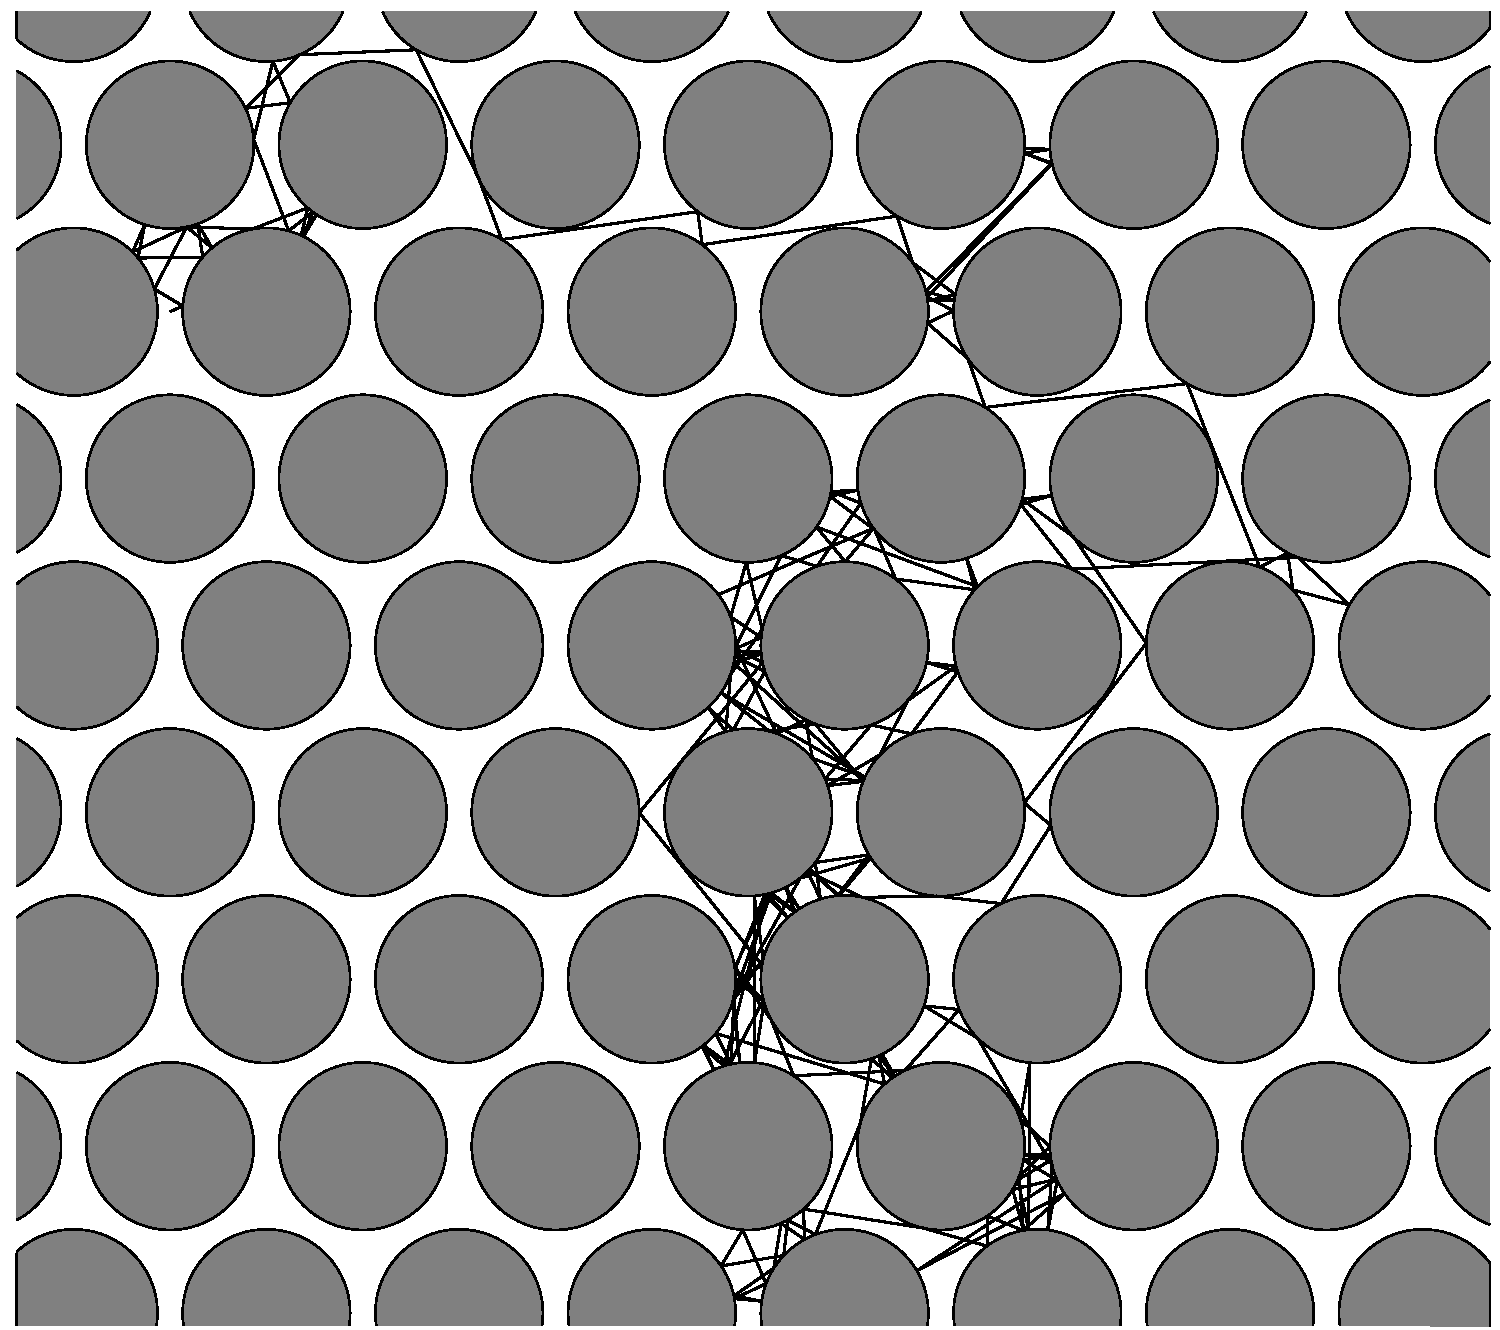
\includegraphics[width=0.45\textwidth]{diffuseChaoticBouncing}
    (b)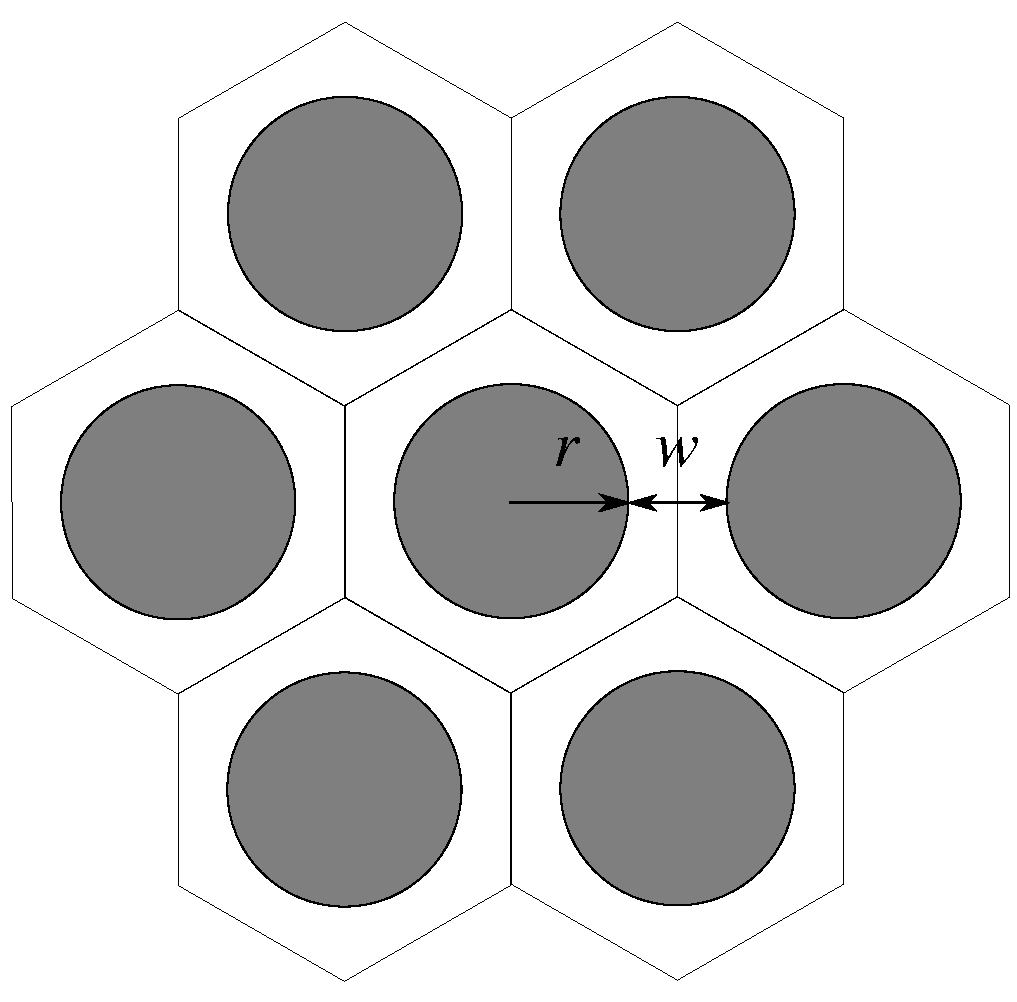
\includegraphics[width=0.45\textwidth]{diffuseLorentzGasParams}
  \end{center}
  \caption[]{\label{fig-chaoticBouncing} Motion in the Lorentz gas system. (a)  The chaotic trajectory of a ``gas'' particle bouncing in the array of disks  arranged in a hexagonal lattice pattern. The distance between disks are close  enough such that the particle has no infinite free flight (finite horizon).  (b) A portion of the triangular Lorentz gas    system. The ratio of distance $w$ between the nearest pair of disks to the    disk radius $r$ determines the dynamical properties in the system. }
\end{figure}

The $2$\dmn\ Lorentz gas is an infinite scatterer array in which diffusion of a light molecule in a gas of heavy scatterers is modeled by the motion of a point particle in a plane bouncing off an array of reflecting disks. The Lorentz gas is called ``gas'' because one can equivalently think of it as consisting of any number of point-like fast ``light molecules'' interacting only with the stationary ``heavy molecules'' and not among themselves.  As the scatterer array is built up from only defocusing concave surfaces, it is a pure hyperbolic system, and one of the simplest nontrivial dynamical systems that exhibits deterministic diffusion, \reffig{fig-chaoticBouncing}.

% The original Lorentz gas assumed a random distribution of heavy
% scatterers; in this case a probabilistic description is unavoidable.

\subsection{Periodic orbit theory}

\Po\ theory of deterministic diffusion, introduced in \refrefs{art91,LorentzDiff}, exploits the fact that the periodic Lorentz
gas
can be constructed by putting together
translated copies of an elementary cell.
Therefore quantities characterizing global dynamics, such as
the Lyapunov exponents and the diffusion tensor, can be
computed from the dynamics restricted to the elementary cell,
as shown numerically in \refref{CGS92}.

However, when this elementary cell is
itself invariant under a discrete symmetry group $G$ the lattice can be tiled
into images under $G$ and the lattice translations of a fundamental
domain.


In \refrefs{DasBuch, art91,LorentzDiff,CGS92,Artuso94} it was shown that deterministic diffusion tensor in the {\em periodic} Lorentz gas can be expressed in terms of (relative) \po s, and exact \cycForm\ for such global dynamical averages as Lyapunov exponent and diffusion tensor were derived, using only the dynamics in the elementary cell. For any dynamical system that has translational symmetry,the full state space $\hM$ (i.e., both spatial coordinates and momenta) has aperiodic tiling
\beq
\hM=\bigcup_{ \hn \in T} \pS_{\hn},
\eeq
by {\em translating} $\pS_{\hn}$ of an {\em elementary cell} $\pS$, with $T$ the abelian group of lattice translations.

In the context of Lorentz gas system, the elementary cell is the hexagonal region centered at the scatterer, see \reffig{fig-chaoticBouncing} (a). The dynamics restricted inside the elementary cell is understood as the periodic boundary condition: when the particle leaves the edge of the hexagon cell, it immediately enters the region again from the opposite edge. We distinguish two types of diffusive behavior; the {\em infinite horizon} case, which allows for infinite length flights, and the {\em finite horizon} case, where any free particle trajectory must hit a disk in finite time. The transition between horizon and infinite horizon is controlled by the ratio of $w/r$, where $w$ is the gap between nearest pair of disk and $r$ the radius of the disk.

We now relate the dynamics in $\pS$ to diffusive properties of the Lorentz gas in $\hM$. Let $\hx(t)\,=\,\hflow{t}{\hx_0}$ denotes the point in the global space $\hM$ reached by the flow in time $t$. $x(t)\,=\,\flow{t}{\xInit}$ denotes the corresponding flow in the elementary cell; the two are related by

\beq
\hn_t(\xInit)=\hflow{t}{\xInit} - \flow{t}{\xInit} \in T \,,
\ee{l-diff-hatn}
the translation of the endpoint of the global path into the elementary cell $\pS$.

Fix a vector $\beta \in \reals^d$, where $d$ is the dimension of the{\statesp}. We will compute the diffusive properties of the Lorentz gas from the leading eigenvalue of the Rulle-Frobenius-Perron \evOper\
\beq
\eigenvL(\beta)\,=\, \lim_{t \rightarrow \infty} \frac{1}{t} \log \langle
e^{\beta \cdot (\hx(t) -x) } \rangle_\pS ~, \quad
\label{eq-diff-1}
\eeq
where the average is over all initial points in the elementary cell, $x \in\pS$. If all odd derivatives vanish by symmetry, there is no drift and the second derivatives
\begin{widetext}
\beq
2d D_{ij} = \left . {\frac{\partial}{\partial \beta_i}} {\frac{\partial}
{\partial \beta_j}} \eigenvL(\beta)\right\vert_{\beta=0} \,=\,\lim_{t\rightarrow
\infty} {\frac{1}{t}} \langle {(\hx(t) -x)_i (\hx(t) -x)_j } \rangle_\pS ~,
\eeq
\end{widetext}
yield a diffusion matrix.  This symmetric matrix can, in general, be anisotropic(\ie, have $d$ distinct eigenvalues and eigen\-vectors). The spatial diffusion constant is then given by the Einstein relation
\beq
D\,=\,{1\over 2 d} \sum_i \left .{{\partial}^2 \over {\partial
      \beta^2_i}} \eigenvL(\beta)\right |_{\beta=0} \,=\,
\lim_{t\rightarrow \infty} {1\over{2d t}} \langle {(\hat{q}(t) -q)^2 }
\rangle_\pS~ ~,
\eeq
where the $i$ sum is restricted to the spatial components $q_i$ of the{\statesp} vectors $x=(q,p)$, \ie, if the dynamics is Hamiltonian, the sum is over the $d$ degrees of freedom.

% PC{reinstate mass, velocity, size to get $\beta$, $m$, $\sigma
% dependencies right}

We now turn to the connection between diffusion and periodic orbits in the elementary cell. It was shown in \refref{CGS92} that the ensemble average in\refeq{eq-diff-1} can be written as an integral over the elementary cell
\beq
\langle e^{\beta\cdot(\hx(t)-x)} \rangle
   = \frac{1}{\vert \pS \vert}\int_{x,y\in \pS} dxdy {\cal L}^t(y,x),
\eeq
given the linear \evOper operator
\beq
{\cal L}^t(y,x) = e^{\beta\cdot(\hx(t)-x)}\delta(y-x(t))
\label{eq-eOper}
\eeq
The interesting dynamical averages is determined by the spectrum of the operator
\beq \det(\eigenvL - \Lop) \,=\,\prod_{p} \exp \left(
  - { \sum_{r=1}^\infty {1 \over r} { e^{(\beta \cdot \hn_p- s
        \period{p}) r} \over \oneMinJ{r} }
  } \right) \,,
\ee{lor-diff-14}
or the corresponding \dzeta\
\beq
1/\zeta(\beta, s)\,=\,\prod_{p}\left( 1 - \frac{e^{(\beta \cdot \hn_p-
      s \period{p})}}{|\ExpaEig_p|} \right) ~,
\label{zeta-diff}
\eeq
where $\period{p}$ is the period of the cycle and $\ExpaEig_p$ the product of expanding eigenvalues of the cycle\rf{DasBuch}.

The \dzeta\ \cycForm\ for the diffusion constant, zero mean drift
$ \expct{ \hat{x}_i } = 0 \,, $ is given by
 \beq D \,=\,{1 \over 2 d}
{ \expct{\hat{x}^2}_\zeta \over \expct{\period{}}_\zeta } \,=\,{1
  \over 2 d } \, {1 \over \expct{\period{}}_\zeta} \sumprime
\frac{(-1)^{k+1} (\hn_{p_1}+ \cdots+ \hn_{p_k})^2}
{|\ExpaEig_{p_1}\cdots \ExpaEig_{p_k}|} \, ,
\label{eq-ecDiffCoef}
\eeq
where the sum is over all distinct non-repeating combination of prime cycles (in the elementary cell). The derivation is standard, still the formula is strange.Diffusion is unbounded motion across an infinite lattice; nevertheless, the reduction to the elementary cell enables us to compute relevant quantities in the usual way, in terms of periodic orbits.

\subsection{Cycles in the elementary cell}
\begin{figure}
  \begin{center}
    (a)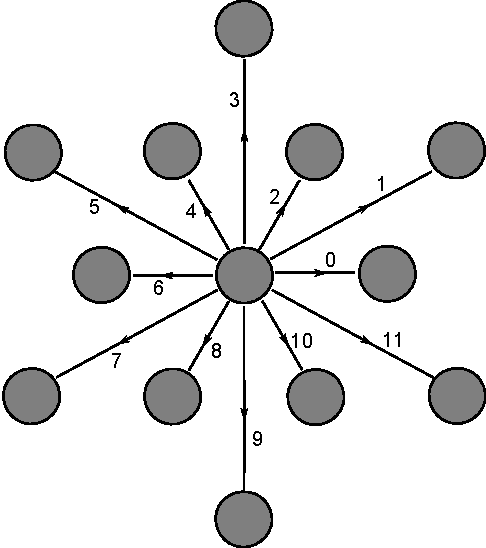
\includegraphics[width=0.27\textwidth]{diffuseDiskDirectionsElCell}
    (b)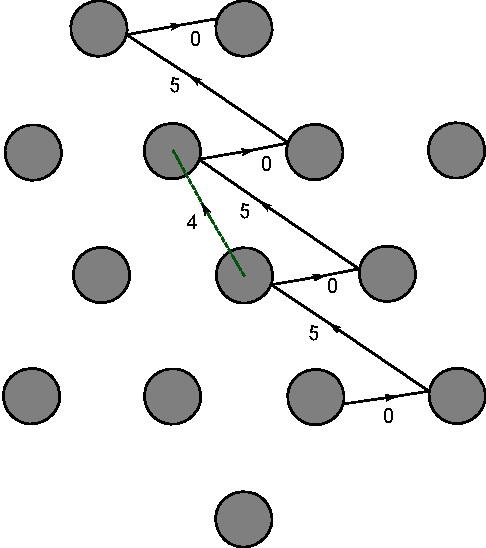
\includegraphics[width=0.27\textwidth]{diffuseDiskDirecsElCell05}
    (c)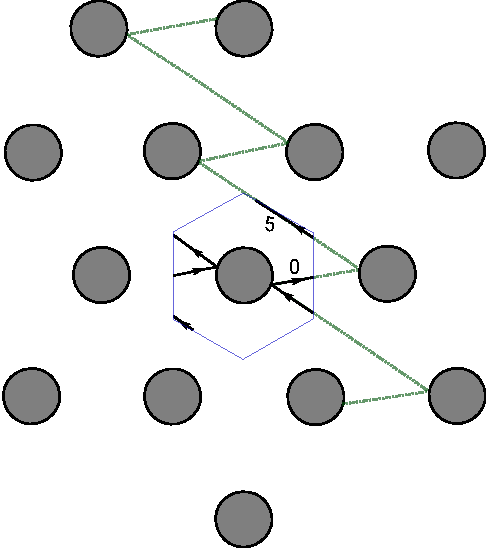
\includegraphics[width=0.27\textwidth]{diffuseDiskDirecsElCell05red}
  \end{center}
  \caption{ Elementary cell symbolic dynamics is obtained by labeling the  translation vectors connecting the center of the current disk to the center of  the next disk. (a) The finite horizon is here imposed by limiting jumps from  the center cell to only the short jumps (six even labels $0, 2,\cdots,10$) and  the `long jumps' (six odd labels $1, 3,\cdots,11$). (b) Running mode  \cycle{05} advances by $\hn_4$ per period. (c) In the elementary cell this is  a \po\ \cycle{05} of topological length 2.  }
  \label{fig-diskDirectionsElCell}
\end{figure}

We use the symbolic dynamics developed in \refref{CGS92} and briefly review the concepts here. With imposed finite horizon there are 12 possible ways of jump from a disk (\reffig{fig-diskDirectionsElCell}\,(a)). Any trajectory in the full space can always be constructed from a series of flights, each belongs to  the 12 ``signature jumps''. In particular, a periodic orbit in the elementary cell is represented as a repeatable string of such symbols. For example, the bouncing mode between nearest disks is written as \cycle{06}, meaning that the periodic orbit is consisted of two successive flights, one traveling towards right (symbol $0$) and the next reflecting backwards (symbol $6$).

Periodic orbits in the elementary cell can either be stationary in the full space that goes back to its original place after completing a full cycle (e.g., \cycle{06} that represents the bouncing of the particle between two nearest disk); or can be in a running mode that generates a net displacement along the trajectory (e.g., \cycle{05}, \reffig{fig-diskDirectionsElCell}\,b and c). The stationary cycles ``trap'' the  particle locally for a finite amount of time while the running cycles advance it. The final diffusion \refeq{eq-ecDiffCoef} can be conceptually understood as the result of competition between the two type of cycles.

With the symbolic dynamics, we then use the least action principle to compute the periodic orbits\rf{DasBuch}. In a planetary Hamiltonian billiard system, the Maupertuis' principle indicates that the traveling length along a cycle is minimized. We can solve the problem by optimizing the total free flight distance with the constraint that links have to connect the specific disks visited along the orbit.

Elementary cycles found using this method and the corresponding cycle expansion calculation results are listed in \reftab{TCELL1}. Although the diffusion coefficient computed using elementary cycles up to $n_p = 8$ matches the numerical experiment value $0.25$, the convergence is not promising.

\begin{table}[htbp]
%\begin{center}
\begin{tabular}{|r|r|r|l|l|}
\hline
${n_p}$ & \# cycles & $\zeta$(0,0) & $\lambda$ & D \\ \hline\hline
1      & 0      &   -    &   -  &   - \\
2      & 24     & -0.31697 & 1.330 & 0.375\\
3      & 64     & -0.54152 & 1.435 & 0.339\\
4      & 168    & -0.09764 & 1.902 & 0.284\\
5      & 516    &  0.02334 & 2.324 & 0.215\\
6      & 1589   & -0.00481 & 1.975 & 0.133\\
7      & 5700   & -0.01241 & 1.885 & 0.184\\
8      & 20729  & -0.01006 & 1.785 & 0.247\\ \hline

\end{tabular}
\caption{\label{TCELL1}
Cycle expansion results computed Schreiber 1992 calculation\rf{CGS92} (and
  this paper) in elementary cell.
}
\end{table}

\section{Into the fundamental domain}
\label{s-SymmetryReduction}
\begin{figure}[htbp]
  \begin{center}
    (a)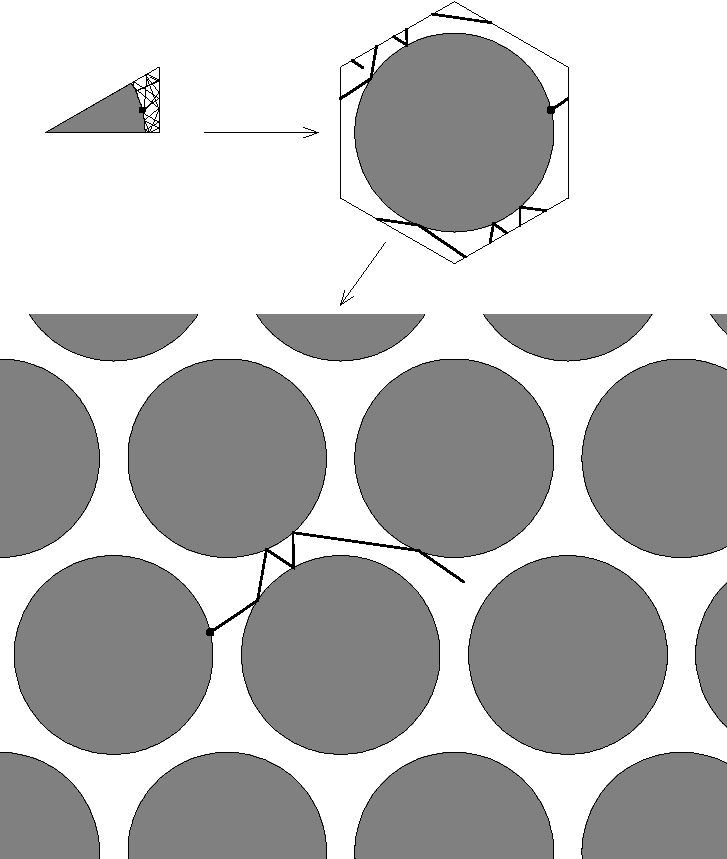
\includegraphics[width=0.45\textwidth]{diffuseSchreiberFig1}
    (b)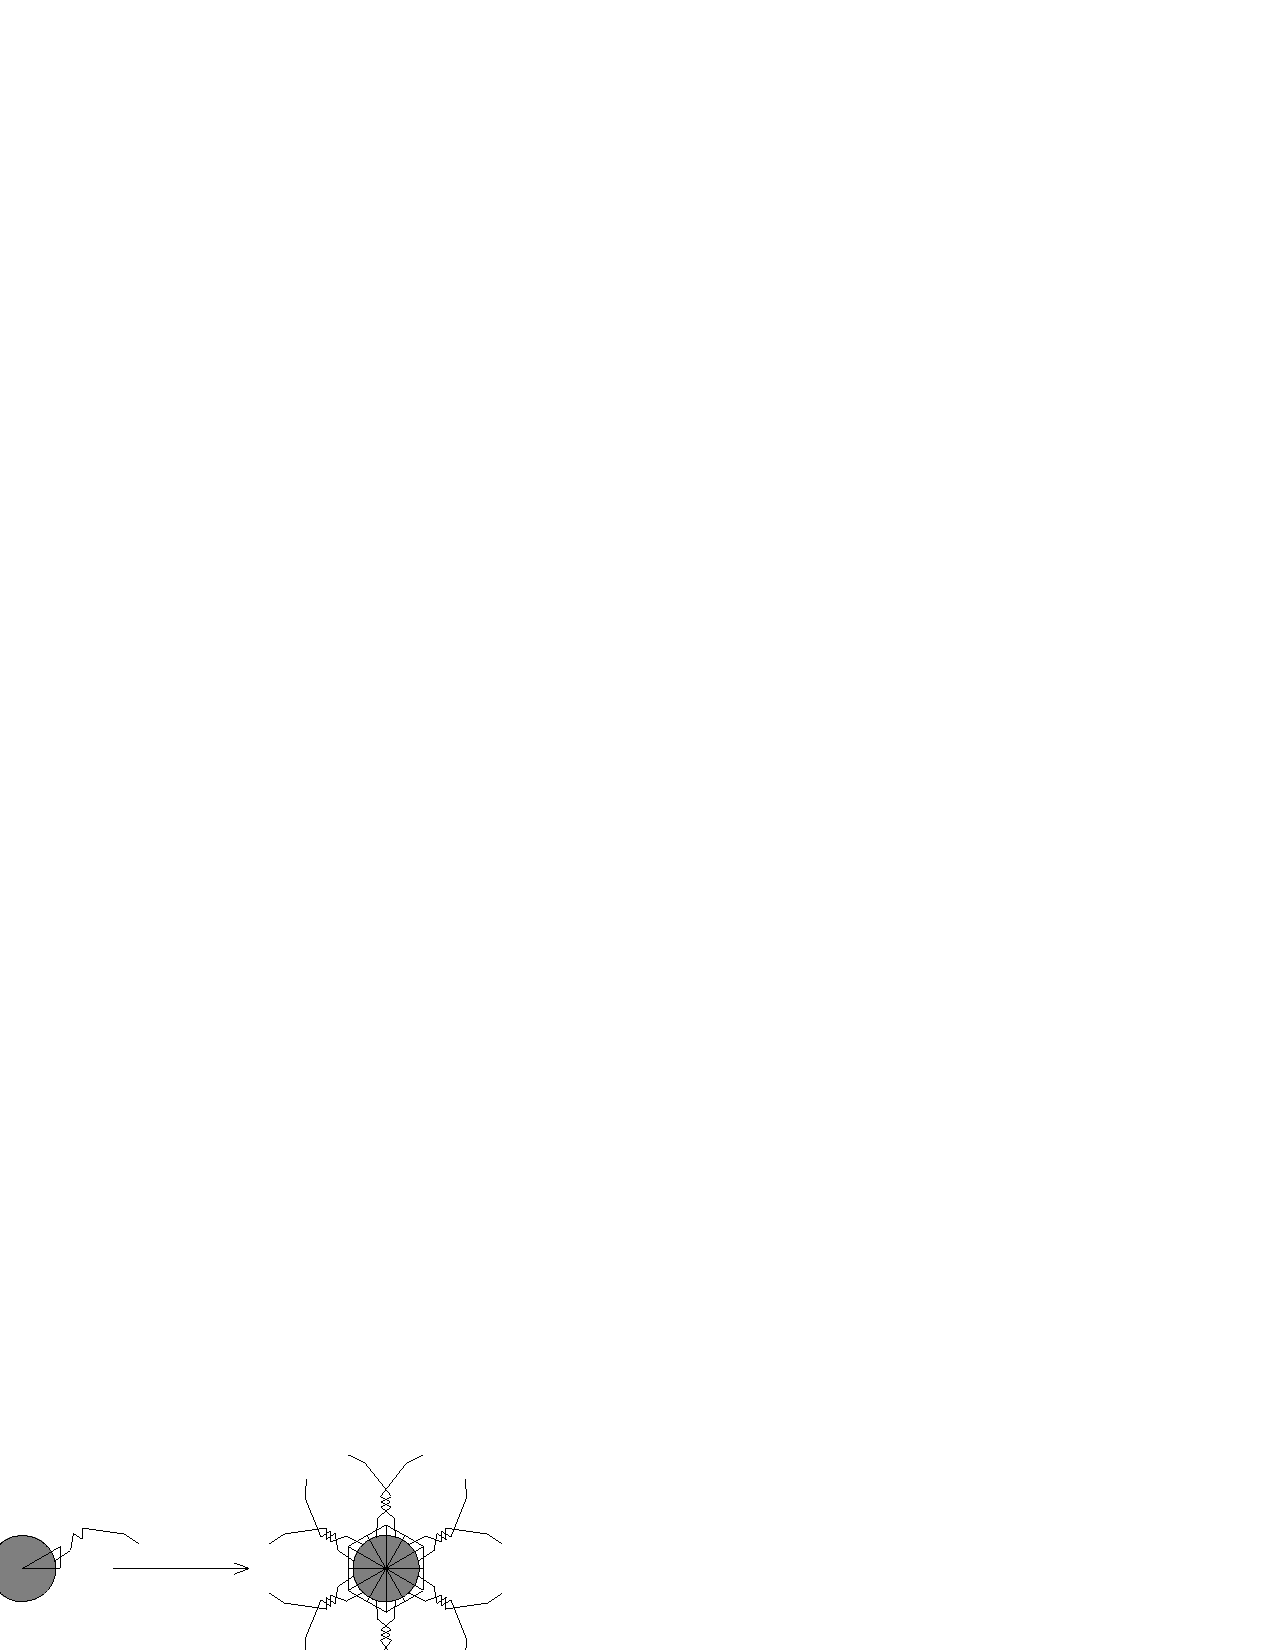
\includegraphics[width=0.45\textwidth]{diffuseSchreiberFig2}
  \end{center}
  \caption[]{\label{fig-schrieberFig12} (a) Motion in the fundamental domain (top left), elementary cell (top right) and  in full space (bottom). (b) An (unwrapped) trajectory (in full  space) and its 12 copies after applying point group actions to it.   }
\end{figure}

%\begin{figure}[htbp]
%  \begin{center}
%    (a)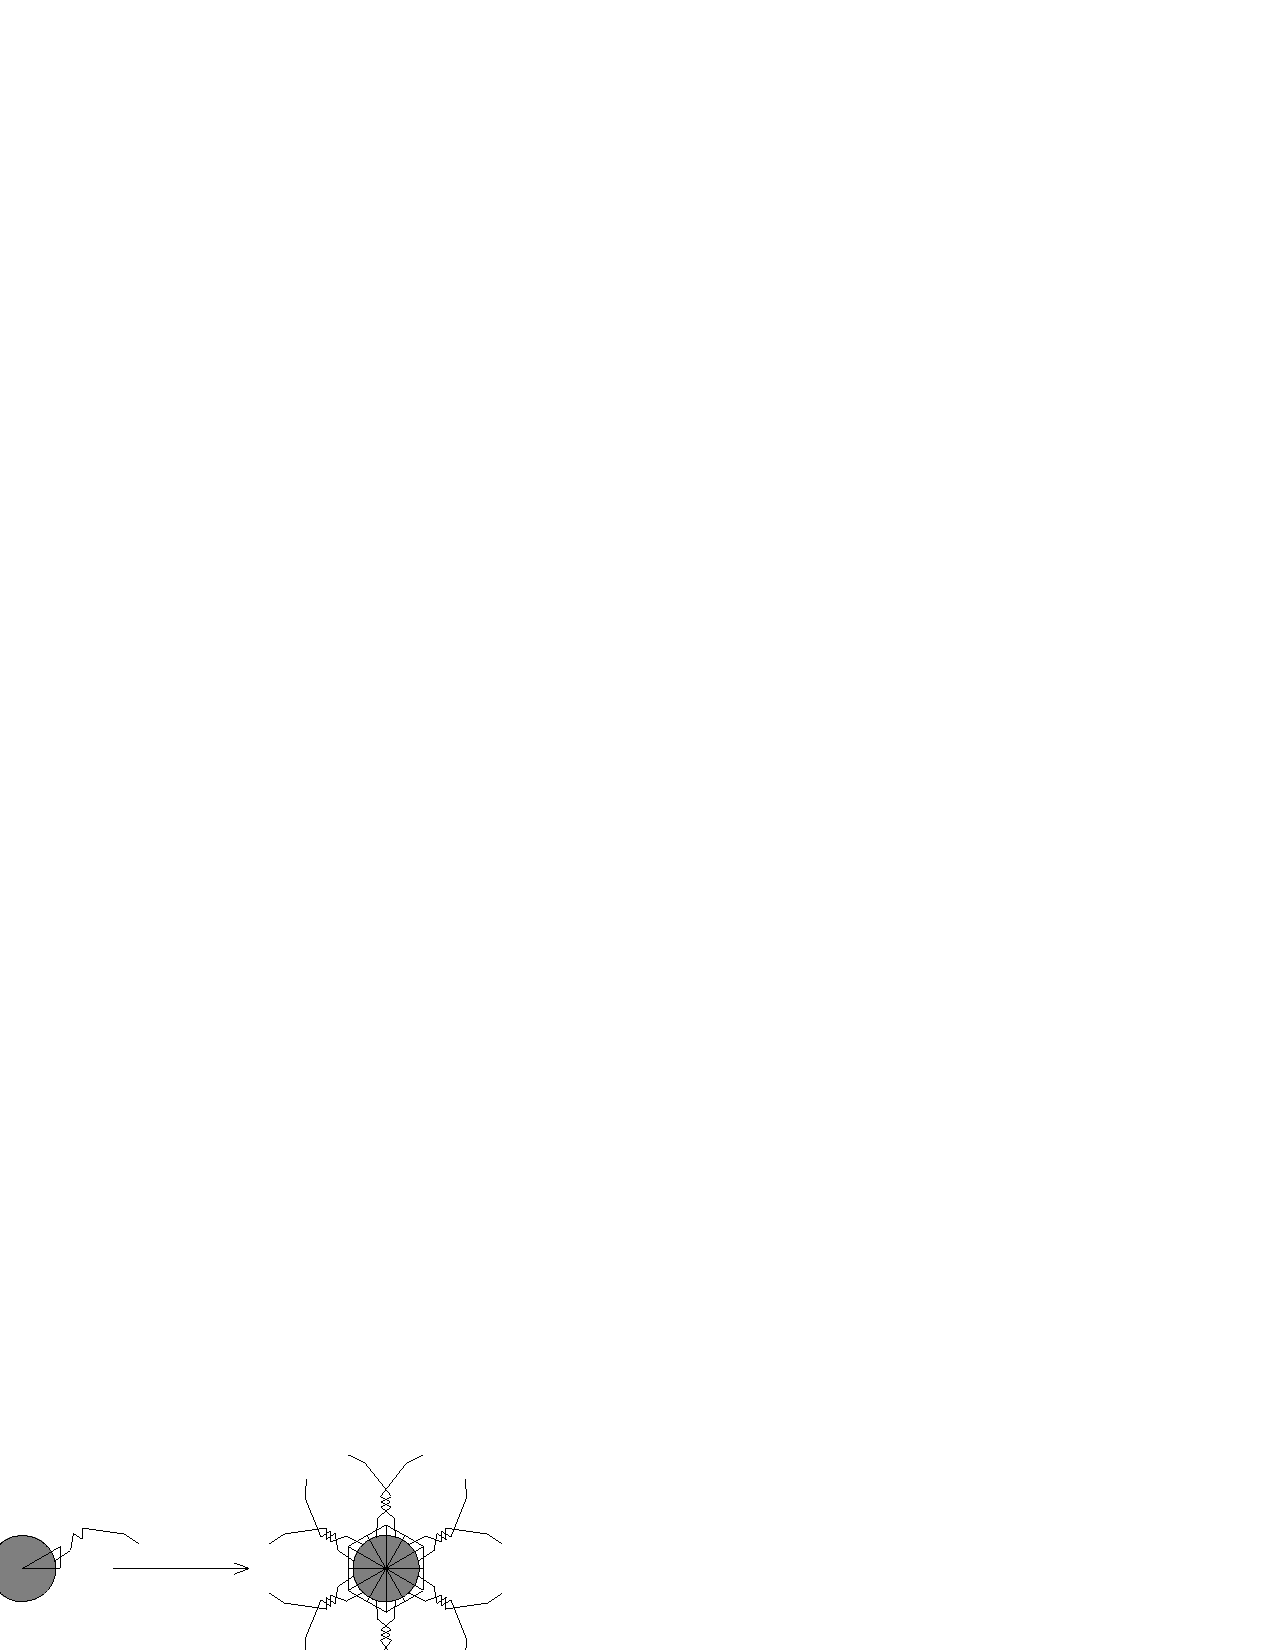
\includegraphics[width=0.45\textwidth]{diffuseSchreiberFig2}
%    (b)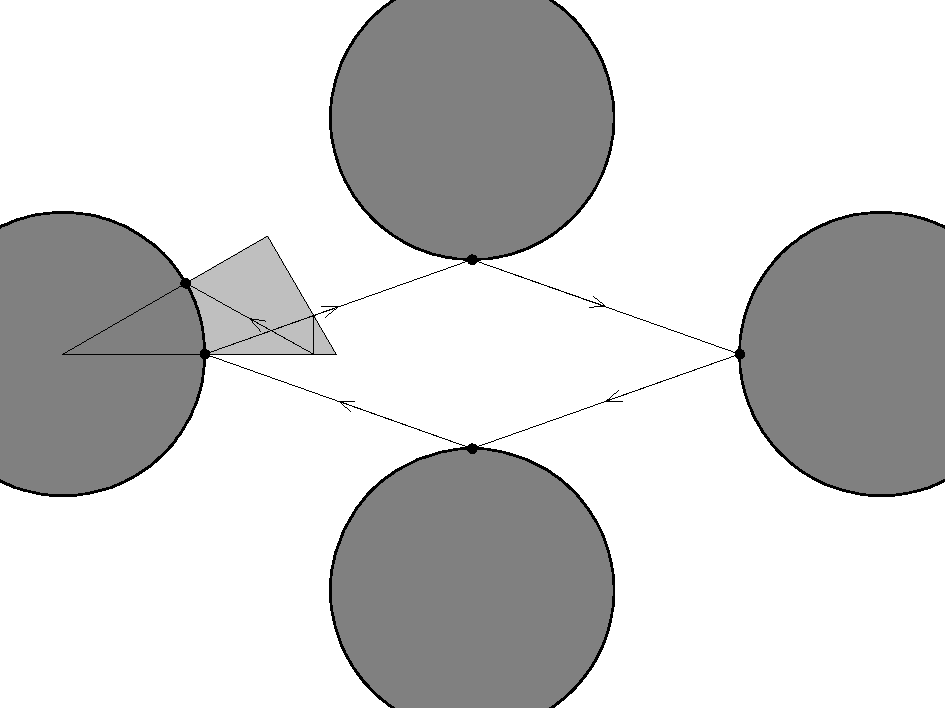
\includegraphics[width=0.45\textwidth]{diffuseSchreiberFig3}
%  \end{center}
%  \caption[]{ \label{fig:schrieberFig23} (a) An (unwrapped) trajectory (in full
%  space) and its 12 copies after applying point group actions to it. (b)
%  Multiplicity of periodic orbits in fundamental domain.}
%\end{figure}

When the scattering array has further discrete symmetries, such as reflection symmetry, each elementary cell may be built from a {\em fundamental domain} ${\widetilde \pS}$ by the action of a discrete (not necessarily abelian) group $G$. The quantity $\tx(t)\,=\,\tflow{t}{\tx}$ denotes the flow in the fundamental domain ${\widetilde \pS}$; $\tflow{t}{\tx}$ is related to$\flow{}{\tx}$ by a discrete symmetry $g \in G$ which maps $\tx(t)\in{\widetilde \pS}$ to ${x}(t) \in {\pS}$. The full $\hM \rightarrow {\widetilde\pS}$ reduction is complicated by the non-abelian nature of $G$, and will be illustrated in this section in detail.

\subsection{How point group changes translation}

In the fundamental domain, one has to realize a few facts before proceeding to the cycle expansion derivation. A point $x$ in the elementary cell can be uniquely identified by its ``mirror image'' in the fundamental domain:
\beq
x=g\circ\tx,
\eeq
given a group action $g\in G$ the discrete symmetry group. In the triangular periodic Lorentz gas the underlying point group is $C_{6v}$ (isomorphic to $D_6$), and the hexagonal elementary cell is partitioned into 12 identical triangular domains. We have to appreciate that the flow $\hat{\phi}^t$ is G-equivariant under the lattice group symmetry, and proceed with the argument that the displacement in full space is also equivariant under the point group symmetry (which is a subset of the lattice group):
\beq
\hn_t(x)\equiv\hn_t(g\circ\tx)= g\circ\hn_t(\tx).
\eeq

We can apply this fact to the displacement associated with a prime periodic orbit $\tp$ restricted in the fundamental domain. Let$\tp\equiv\{\tx_0,\tx_1,\ldots,\tx_{N_\tp}\}$, with topological length $N_\tp$and $\tx_i$ the bouncing points on the orbit. For each flight (e.g. from $\tx_i$to $\tx_{i+1}$) we denote the associated displacement in full space $\hn(\tx_i,e)$. However, one has to be careful when adding the individual displacements together when moving along a fundamental domain orbit. Unlike in elementary cell, the fundamental domain point $\tx_i$ does not distinguish in which triangular piece it is. Instead, we assign a point group element$g_\tp(\tx_{i+1},\tx_{i})$ to keep track of changes in absolute orientation. We now write the displacement traveled along the orbit, after finishing a full cycle:
\beq
\hn_{\tp}(\tx_{0})=\sum_{i=0}^{N_\tp-1}\hn(\tx_{i},g_{\tp,\tx_0}(\tx_{i}))=\sum_{i=0}^{N_\tp-1}g_{\tp,\tx_{0}}(\tx_{i})\circ\hn(\tx_{i},e),
\eeq
where $g_{\tp,\tx_{0}}(\tx_i)=\prod_0^{j-1} g_\tp(\tx_{j+1},\tx_{j})$ is the accumulated orientation changes along the orbit when starting from $\tx_{0}$.The displacement now has its dependence on the starting point we choose. We denote the total group action for the orbit

\bea
h_{\tp}(\tx_i)&\equiv& g_\tp(\tx_{i},\tx_{i-1})\circ\ldots\circ
g_\tp(\tx_{0},\tx_{N_\tp-1})\nonumber\\
&& \circ g_\tp(\tx_{N_\tp-1},\tx_{N_\tp-2})\circ \ldots\circ
g_\tp(\tx_{i+1},\tx_{i}),
\eea
which one can immediately see the connection $\flow{t_\tp}{\tx_i}=h_{\tp}(\tx_i)\tflow{t_\tp}{\tx_i}$. Although the group action $h_{\tp}(\tx_i)$ depends on the initial points on the orbit, it is a property of the orbit's symmetry, and subsequently all $h_{\tp}(\tx_i), \tx_i\in\tp$ belong to the \emph{same} subgroup of $G$.

We also want to define the quantity:
\beq
\hat{L}_{\tp}^{r}(\tx_i)\equiv
(e+\hp^{1}(\tx_i)+\cdots+\hp^{r-1}(\tx_i))\cdot\hn_{\tp}(\tx_i),
\label{eq-fdDisplacement}
\eeq
to be the displacement traveled along the orbit $r$ times, starting from $\tx_i$.  Though one may not appreciate immediately, \refeq{eq-fdDisplacement} takes care of the rotational symmetry that does not commute with translation, and we will show that it gives the proper displacement needed for computing diffusion coefficient in the fundamental domain.


\subsection{Gymnastics of equations}

We properly treat the discrete symmetry by projecting the trace of\evOper \refeq{eq-eOper} to the group's subspace:
 \bea
\tr{\cal L}^t &=& \sum_{\alpha \in\II_G} \tr{\cal L}_{\alpha}^t\nonumber\\
\tr{\cal L}_{\alpha}^{t} &=& \frac{d_\alpha}{|G|}\sum_{\sigma \in
  G}\sum_{h\in G}\chi_\alpha(h)\int_{\t {\cal M}} d\tx \delta (h\tx -
\flow{t}{\tx})e^{\beta\cdot\sigma\cdot\hn^t(\tx)}.\nonumber\\
\label{eq-traceSum}
\eea

The delta function part $\delta (h\tx - \flow{t}{\tx})$ in the integral selects the fundamental domain periodic points that satisfy the group condition $h\equiv h^r_{\tp}(\tx_i)$. The displacement traveled starting from each of those points and along the orbit $r$ times takes the form already computed in\refeq{eq-fdDisplacement}. The rest is straight forward gymnastics of algebra,which yields the dynamical zeta function for the $\alpha$ irreducible representation:
\begin{widetext}
 \beq
\frac{1}{\zeta_{\alpha}(\beta,s,z)}
=\exp\left(-\frac{d_\alpha}{|G|}\sum_{\sigma\in
G}\sum_{\tp}\frac{1}{N_{\tp}}\sum_{\tx_{i}\in\tp}\sum_{r=1}^{\infty}\frac{t_{\tp}^{r}}{r}\chi_{\alpha}(\hp^{r}(\tx_i))e^{\beta\cdot\sigma\cdot\hat{L}_{\tp}(r,\tx_i)}\right),
\label{eq-fdZeta}
\eeq
\end{widetext}

where
 \beq t_{\tp}\equiv
\frac{z^{N_{\tp}}e^{-sT_{\tp}}}{|\ExpaEig_\tp|}, \eeq

is the ``weight'' associated to the orbit. Equation \refeq{eq-fdZeta} differsfrom its counterpart in elementary cell, but can be reduced to if the symmetry group contains only $e$.

We are interested in the one dimensional, symmetric trivial representation with$ d_\alpha = 1 $ and all $ \chi(h) = 1 $; there by we drop the subscript $\alpha $ in the following calculation. Partial derivative with respect to$\beta$ gives:
\begin{widetext}
\bea
\frac{\partial^{2}}{\partial\beta^{2}}\frac{1}{\zeta(\beta,s,z)}
&=\frac{1}{\zeta(\beta,s,z)}\left(\left(\frac{1}{|G|} \sum_{\sigma\in G}\sum_{\tp}\sum_{\tx_i\in \tp}\sum_{r=1}^{\infty}\frac{\sigma\cdot \hat{L}_{\tp}^{r}(\tx_i)t_{\tp}^r e^{\beta\cdot\sigma\cdot \hat{L}_{\tp}^{r}(\tx_i)}}{N_{\tp}r}\right)^{2}\right.\nonumber\\
&\left.-\frac{1}{|G|}\sum_{\sigma\in G}\left(\sum_{\tp}\sum_{\tx_i\in
      \tp}\sum_{r=1}^{\infty}\frac{\vert \sigma\cdot
      \hat{L}_{\tp}^{r}(\tx_i)\vert^{2}t_{\tp}^{r}e^{\beta\cdot\sigma\cdot
        \hat{L}_{\tp}^{r}(\tx_i)}}{N_{\tp}r}\right)\right).
        \eea
\end{widetext}
The first term in the formula corresponds to $ \langle\hx\rangle^2 $ and
second to $ \langle\hx^2\rangle $. It is trivial to see that
\beq\sum_{\sigma\in G}\frac{\sigma\cdot
  \hat{L}_{\tp}^r(\tx_i)t_{\tp}^r e^{\beta\cdot\sigma\cdot
  \hat{L}_{\tp}(r,\tx_i)}}{N_{\tp}r} \equiv 0,
\eeq
because of the summation over the discrete group $G$. Thus the calculated mean drift is zero, consistent with the symmetry of the system. Observing that the length$\vert \sigma\cdot \hat{L}_{\tp}^{r}(\tx_i) \vert$ does not change under rotation, we write
\bea
\langle\hx^2\rangle &=& \left.\frac{1}{\zeta(\beta,s,z)}\sum_{\tp}\sum_{r=1}^{\infty}\frac{t_{\tp}^{r}}{r}\sum_{\tx_i\in \tp}\frac{\vert\hat{L}_{\tp}^{r}(\tx_i)\vert^{2}}{N_{\tp}}\right\vert_{\beta=0,s=0, z=1} \nonumber\\
&=& \left.\prod_{\tp}\left(1-\frac{z^{N_{\tp}}}{\vert\ExpaEig_\tp\vert
    }\right)\sum_{\tp}\sum_{r=1}^{\infty}\left(\frac{z^{N_{\tp}}}{\vert\ExpaEig_\tp\vert
    }\right)^r\frac{\vert\hat{L}_{\tp}^{r}\vert^2}{r}\right\vert_{z=1}
\label{eq-meanSquareDisp}
\eea with $\hat{L}_{\tp}^{r}\equiv\sum_{\tx_i\in
  \tp}\frac{\vert\hat{L}_{\tp}^{r}(\tx_i)\vert^{2}}{N_{\tp}}$ the
average square displacement in full space when traveling along a fundamental domain $r$ times. Formula \refeq{eq-meanSquareDisp} is an infinite polynomial in the auxiliary variable $z$, and should be truncated to the topological length of the longest periodic orbits find in calculation.

\subsection{Grammar of fundamental domain cycle}

\begin{figure}[htbp]
  \begin{center}
    (a) 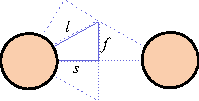
\includegraphics[width=0.35\textwidth]{diffuse7diskFundDflips}
    (b) 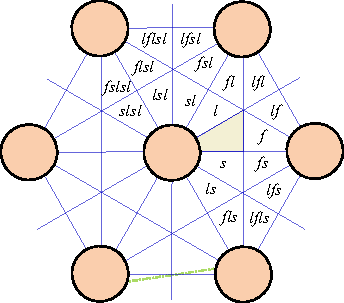
\includegraphics[width=0.35\textwidth]{diffuse7diskFundDtiles}
  \end{center}
  \caption{\label{fig-7diskFundDflips} (a) The three generators of tiling of the  plane by a fundamental domain: two generators of \Dn{12} tiling, reflection  $s$ across the short disk-disk separation, reflection $\ell$ across the long  disk-disk separation; and a translation generator $f$ that pivots (`flips') a  disk center to disk center by flip across the symmetry line normal to the short disk-disk separation. (5) Tiling of the 7-disk by copies of the fundamental domain, labeled by a (not unique) sequence of the three generators  $\{s,\ell,f\}$, chosen so that each sequence contain one and only on  disk-to-disk pivot $f$. }
\end{figure}
    \TZ{2015-10-19}{I do not really use the three generators to compute the fundamental domain cycles, instead I use the idea of topological distinct flights (\reffig{fig-fdflights}). We have yet to discuss the equivalence between the 3-generators and topological distinct flight in the two  figures. }

\begin{figure}[htbp]
  (a)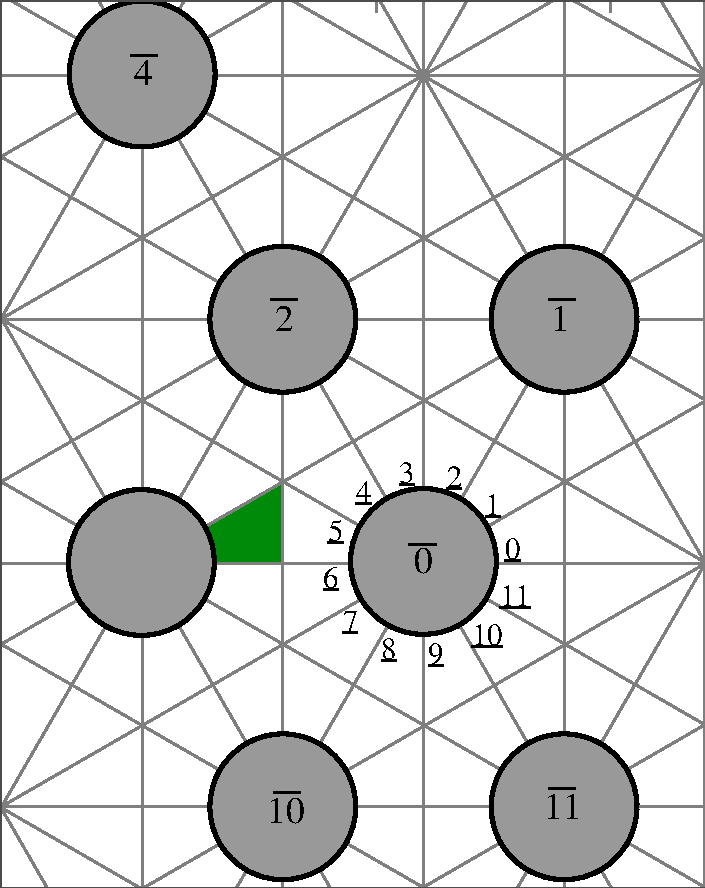
\includegraphics[width=0.35\textwidth]{diffuseFDSymbolIllustration}
  (b)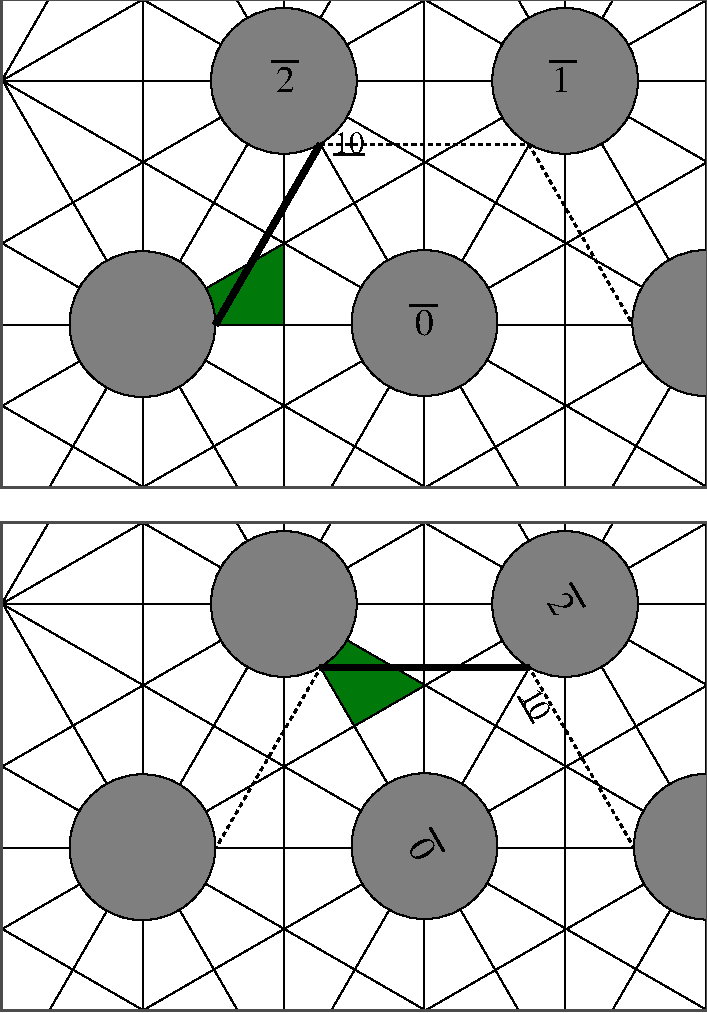
\includegraphics[width=0.35\textwidth]{diffuseFDSymbolOrbits}

  \caption{\label{fig-fdflights} Fundamental domain symbolic dynamics. (a) With  imposed finite horizon and starting on the edge of a disk in fundamental  domain (the green filled region), there are at most 6 disks can be reached  without collision (disk  $\overline{0},\overline{1},\overline{2},\overline{4},\overline{10}$ and  $\overline{11}$). Similar to how elementary cell symbolic dynamics are  created, we label the 12 triangular pieces of a disk in a counter clock-wise  manner, from $\underline{0}$ to $\underline{11}$. The combination of a disk  label and a triangular piece label $\{\overline{i},\underline{j}\}$ uniquely  identifies a topologically distinct flight. (b) The fundamental domain fixed   point $\{\overline{2},\underline{10}\}$, which corresponds to a periodic   orbit of length 6 in elementary cell ($\cycle{0246810}$), is unwrapped in   global space. After each collision we re-label the disks and triangular   partitions according to their relative positions to the ``new'' fundamental   domain. In the figure labels are also rotated according to the point   group actions.}
\end{figure}



In the international crystallographic notation, the hexagonal lattice is called $p6mm$, with point group $6mm$, where prefix $p$ indicates that the unit cell is primitive (not centered),
\beq
\Group = \{
e, C_6^+, C_6^-, C_3^+, C_3^-, C_2,
\sigma_{d1}, \sigma_{d2}, \sigma_{d3},
\sigma_{v1},\sigma_{v2}, \sigma_{v3}
\}
\,,
\eeq
with $s=\sigma_{d}$ the reflection across the short disk-disk separation, and $\ell=\sigma_{v}$ reflection across the long disk-disk separation generators of \Dn{12}. The entire space group $p6mm$is then generated by adding a disk-to-disk generator $f$ that pivots a disk center to another by flip across the symmetry line normal to the short disk-disk separation, \reffig{fig-7diskFundDflips}a. We find it convenient to define $C$ as the generator of cyclic rotations by $\pi/3$,
\beq
\ell s = C_6^- = C
\,,\quad
C^6 = e
\,;\qquad
s \ell =  C_6^+
\,,\qquad
s  =  C_6^+ \ell
\,.
\eeq

\TZ{2015-10-22}{The idea is that the topological periodic orbit in the fundamental domain is not sensitive to the order of flips. When $w$ increases, one might notice that a single flight along the orbit changes from $sf$ to $fs$. However, the relative position between the start and end triangular cells are always the same.}

A free flight between two disks in the full space may then be wrapped into fundamental domain, according to the sequence cell edges $\{s,\ell,f\}$ it passed. For example, there are different paths when jump to disk $0$: it can be as simple as a single pivot about $f$, or can be more complex such like $\ell f s$ that involves multiple flips, ~\reffig{fig-7diskFundDflips} b. Although we can associate each free flight with a chain of the generators, some of the combinations are equivalent. The short jump $sf$ is topologically equivalent to $fs$, in the sense that the particle ends up in the same copy of fundamental domain before next collision.

Our task is to generate all distinct itineraries from $\{s,\ell,f\}$. One can immediately realize a partial list of the equivalence relations:
\bea
f s &=& s f
\,,\nonumber\\
f \ell f&=&\ell f \ell
\,.
\eea

All longer equivalence relations in ~\reffig{fig-7diskFundDflips} can be reduced to the above primitive ones:
\bea
f s \ell &=& s f \ell\,,\nonumber\\
\ell f\ell s &=& f \ell s f\,.
\eea

There are also some pruning rules to keep in mind. Because a free flight cannot cross the same border twice, sequences including $\ell\ell,ff,ss$ are forbidden. $C^3$ (and all higher orders) is also pruned as the particle cannot cross the center hard disk; nor swirl around it.

While the string description of flight is mathematically rigorous and accurate, it is practically hard to be encoded into programs for computing the orbits, because the number of equivalent strings increases exponentially when the length (of a single string) increases. However, there is a more physically intuitive way to organize the type of flight, by means of ``topological flight'', \reffig{fig-fdflights} (a). In this representation, a equivalence relation like $sf\equiv fs$ can be uniquely identified by a combination of a disk number and a partition number $\{\overline{0},\underline{6}\}$. Longer flight such like $\ell f \ell s \ell f \equiv  f \ell f s \ell f \equiv f \ell s f \ell f \equiv f \ell s \ell f \ell$ that cross many boundaries now yields a very simple symbol pair $\{\overline{1},\underline{5}\}$.

The topological flight leads to a straight forward numerical scheme to find cycles. The disk number fixes the two ends of the free flight while the partition number limits the range of angles on the disk. Similar to searching cycles in elementary cell, we now have a constrained version of numerical minimization problem which can be solved using standard non-linear optimization approach.

 \TZ{2015-11-02}{I have not yet talked about the pruning rule in detail here; it is more complicated bases on the reflection angle}

\subsection{Diffusion in the fundamental domain}
\begin{table}[htbp]
\hfill
\TZ{2015-10-19}{Do we need this many digits in the table?}
\begin{tabular}{|r|r|r|l|l|}
\hline
$\period{p}$ & \# cycles & $\zeta$(0,0) & $\lambda$ & D \\ \hline\hline
1      & 5      & -0.2169759 & 1.39193 & 0.37795 \\
2      & 10     & -0.0248233 & 1.74541 & 0.23118\\
3      & 33     & -0.0221962 & 1.72235 & 0.25257\\
4      & 108    & -0.0002192 & 1.74450 & 0.24165\\
5      & 373    &  0.0023463 & 1.76079 & 0.24468\\
6      & 1378   &  0.0096330 & 1.75610 & 0.24068\\ \hline\hline
\multicolumn{3}{|l|}{numerical experiment}
                           & 1.760 & 0.25
\\ \hline
\end{tabular}

\caption{\label{TCELL2}
  Results for $w$=0.3. Calculation in FD. Gaspard 1992
  note: ``My numerical estimate for the Lyapunov exponent when $w=0.3$ is
  $\lambda = 1.760 \pm 0.002$, which supports the result of this table.''
}
\end{table}

\begin{figure}[htbp]
  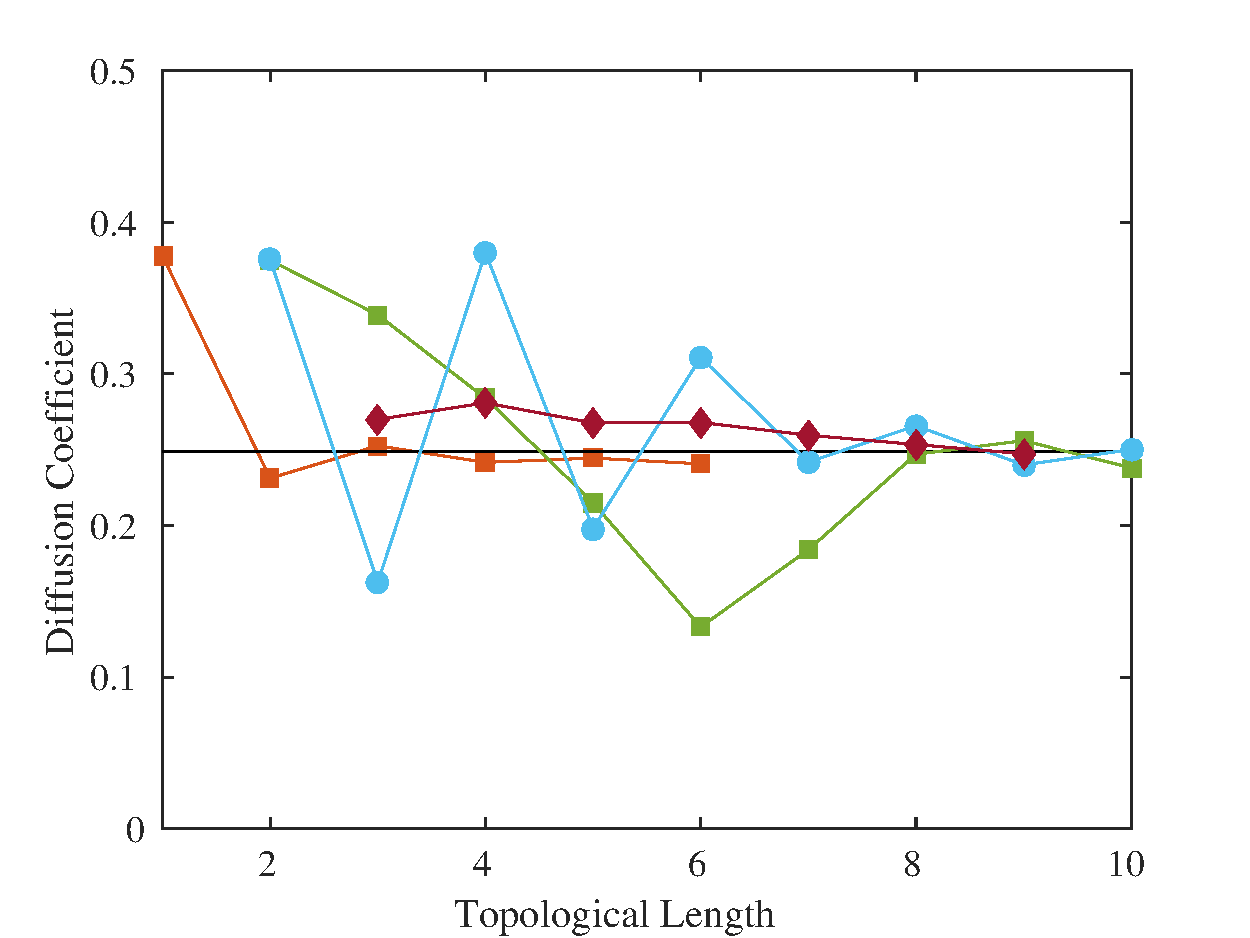
\includegraphics[width=0.45\textwidth]{diffuseCycleExpansionResults}
  \caption[]{\label{fig-convergence} The convergence of diffusion coefficients  calculated using cycle expansion in elementary cell (green squares),  fundamental domain(orange squares). We  also show the convergence of ``periodic orbit expansion'' method, with and  without Shanks transformation (circles and diamonds) discussed in  \rf{Morriss1994}. Here $w = 0.3$.  }
   \TZ{2015-10-19}{Any comment on this?}
\end{figure}

\begin{figure}
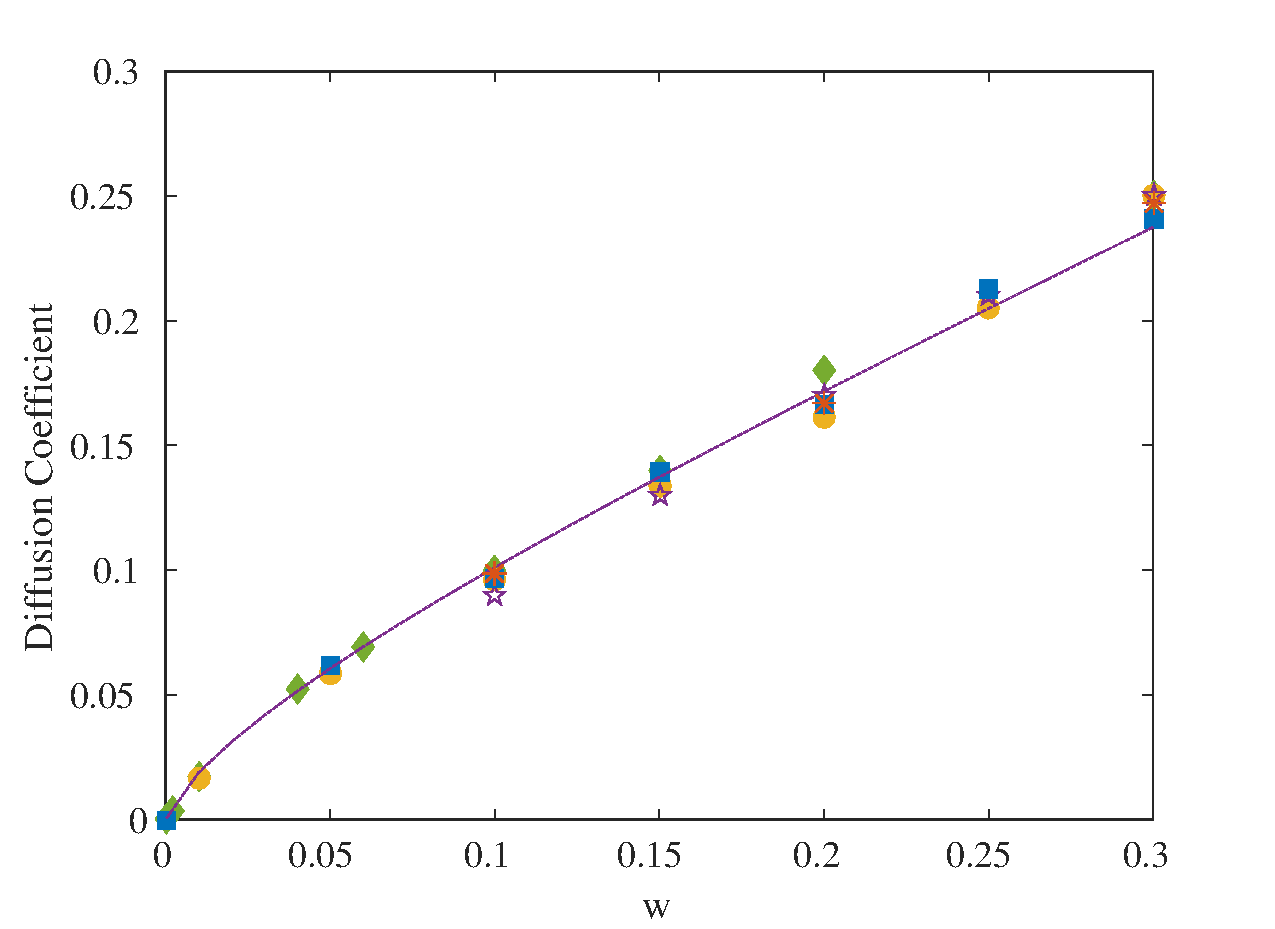
\includegraphics[width=0.45\textwidth]{diffuseDiffCoefPlot}
  \caption[]{\label{fig-results} Diffusion coefficients as a function $w$.  Figure generated using data from various resources. Diamonds are results from  Green-Kubo numerical experiments\rf{MacZwa83}; stars\rf{BaEvCo93} and  circles\rf{GasBar95} are calculated from escape rate; and triangles are  given by Hausdorff fractal dimension calculation\rf{GasBar95}; dashed line  is a statistical approximation\rf{Angstmann20121819}}.
\end{figure}

Compared with various methods, the symmetry reduced cycle expansion method converges the fastest, table \ref{TCELL2} and \reffig{fig-convergence}. Diffusion coefficient computed from $\sim2000$ fundamental domain cycles of topological length up to 6 gives two significant digits, while the elementary cell calculation needs over $\sim 10000$ cycles in order to converge. In other words, the fundamental domain cycles suggests a better and denser partition of the phase space.

\TZ{2015-10-19}{Talk about other two methods}.

To further test \refeq{eq-meanSquareDisp}, we compute the diffusion coefficient for $w/r = 0.05, 0.10, 0.15, 0.20, 0.25, 0.30$, and compare the results with existing numerical experiments and a recent statistical estimation, \reffig{fig-results}. In Green-Kubol velocity auto-correlation method the  diffusion coefficient can be extrapolated to the accurate reference value $0.250$ (at $w/r=0.30$), using ensembles of $10^6\sim10^7$ gas particles flying for long time $T>20$ (and the number of bounces is greater than this)\rf{MacZwa83}. On the other hand, while statistical approach yields a smooth analytical formula\rf{Angstmann20121819}, the diffusion property is fundamentally never a smooth, monotonically increasing function of $w$
\TZ{2015-11-02}{what is that 1D diffusion reference that shows the anywhere continuous, nowhere smooth curve?}. Again, the effectiveness (yet correctness) of the cycle expansion is proved by those comparison.

\section{Conclusion}

 \TZ{2015-11-02}{What else do we put here?}
% Specify following sections are appendices. Use \appendix* if there
% only one appendix.
%\appendix
%\section{}

\begin{acknowledgments}
We are grateful to Pavel M. Svetlichnyy for many fruitful discussions in the early stages of this project, and the key suggestion that the plane can be tiled in terms of three elementary tiling generators. TZ was supported by NSF grant ???-?????. PC thanks to the family of late G. Robinson, Jr. and NSF grant DMS-1211827 for financial support.
\end{acknowledgments}

\ifboyscout
% switch to Private
\newpage
    \input ../tingnan/flotsam
% \newpage
\fi


\bibliographystyle{apsrev4-1}
\bibliography{../bibtex/siminos,../bibtex/diffuse}
% Choosing a journal automatically selects the correct APS BibTeX style
% file (bst file), so only uncomment the line below if necessary.
% \bibliographystyle{apsrev4-1}



\end{document}



% If in two-column mode, this environment will change to single-column
% format so that long equations can be displayed. Use sparingly.
% \begin{widetext}
%   put long equation here
% \end{widetext}

% Use the figure* environment if the figure should span
% across the entire page. There is no need to do explicit centering.

% Surround figure environment with turnpage environment for landscape
% figure
% \begin{turnpage}
%   \begin{figure}
%     \includegraphics{}%
%     \caption{\label{}}
%   \end{figure}
% \end{turnpage}

% Here is an example of the general form of a table:
% Insert the column specifiers (l, r, c, d, etc.) in the empty braces of the
% \begin{tabular}{} command.  The ruledtabular enviroment adds doubled
%   rules to table and sets a reasonable default table settings.  Use
%   the table* environment to get a full-width table in two-column Add
%   \usepackage{longtable} and the longtable (or longtable*}
%   environment for nicely formatted long tables. Or use the the [H]
%   placement option to break a long table (with less control than in
%   longtable).
% \begin{table}%[H] add [H] placement to break table across pages
% \caption{\label{}}
% \begin{ruledtabular}
%   \begin{tabular}{}
% Lines of table here ending with \\
% \end{tabular}
% \end{ruledtabular}
% \end{table}

% Surround table environment with turnpage environment for landscape
% table
% \begin{turnpage}
%   \begin{table}
% \caption{\label{}}
% \begin{ruledtabular}
%   \begin{tabular}{}
% \end{tabular}
% \end{ruledtabular}
% \end{table}
% \end{turnpage}
